% v2-acmtog-sample.tex, dated March 7 2012
% This is a sample file for ACM Transactions on Graphics
%
% Compilation using 'acmtog.cls' - version 1.2 (March 2012), Aptara Inc.
% (c) 2010 Association for Computing Machinery (ACM)
%
% Questions/Suggestions/Feedback should be addressed to => "acmtexsupport@aptaracorp.com".
% Users can also go through the FAQs available on the journal's submission webpage.
%
% Steps to compile: latex, bibtex, latex latex
%
% For tracking purposes => this is v1.2 - March 2012
\documentclass{acmtog} % V1.2
\usepackage{graphicx}
\usepackage{float}
\usepackage{cite}
\usepackage[ruled,lined,boxed,linesnumbered]{algorithm2e}

%\acmVolume{VV}
%\acmNumber{N}
%\acmYear{YYYY}
%\acmMonth{Month}
%\acmArticleNum{XXX}
%\acmdoi{10.1145/XXXXXXX.YYYYYYY}
\acmVolume{28}
\acmNumber{4}
\acmYear{2019}
\acmMonth{September}
\acmArticleNum{106}
\acmdoi{10.1145/1559755.1559763}

\begin{document}

\title{Qlearning for robot navigation in dynamic environments} % title

\author{Changda Tian {\upshape and} Xudong Liu
\affil{CS222 Course Project 2018 fall}
% NOTE! Affiliations placed here should be for the institution where the
%       BULK of the research was done. If the author has gone to a new
%       institution, before publication, the (above) affiliation should NOT be changed.
%       The authors 'current' address may be given in the "Author's addresses:" block (below).
%       So for example, Mr. Fogarty, the bulk of the research was done at UIUC, and he is
%       currently affiliated with NASA.
}


\maketitle


\section{Introduction}
At present, more and more autonomous robots are built to liberate human from doing tedious and
dangerous work. And more and more autonomous robots are walking into people's life. We have intelligent
sweeping robot in our home, and we are watching the autonomous vehicles growing more and more muture.
So autonomous robots are playing an more and more important role in our life.

Generally speaking, an autonomous robot is designed to complete specific tasks
using robot-mounted sensors.Two major problems are required to be solved before
robots can autonomously navigate in dynamic environments: localization and path planning.
\begin{figure}[H]
	\centering
	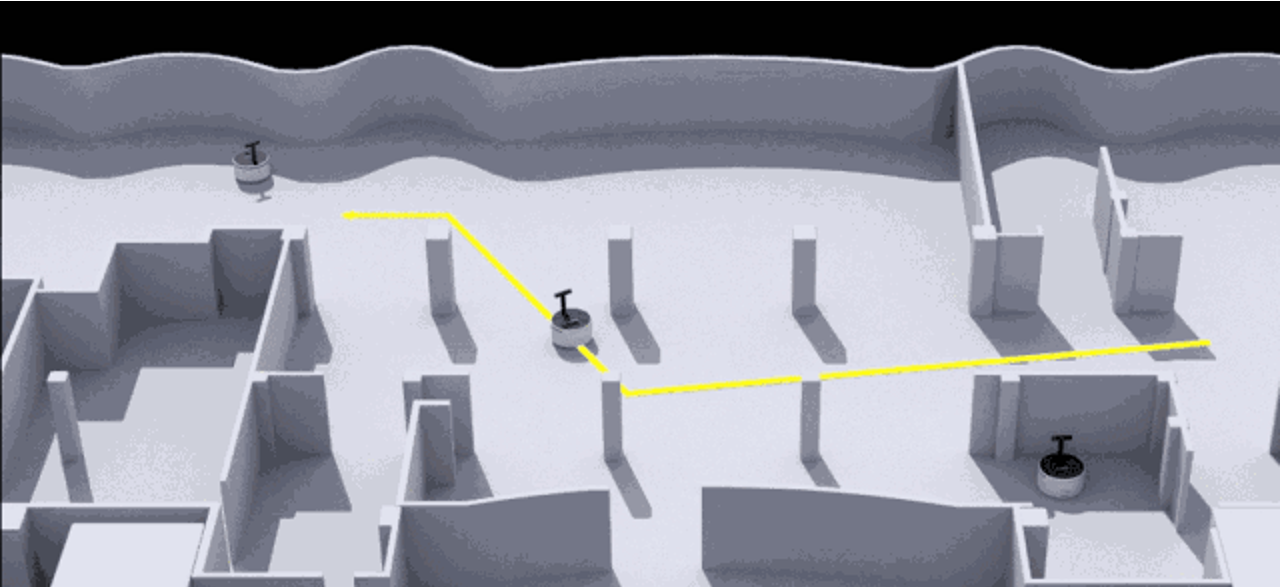
\includegraphics[width=0.3\textwidth]{int.PNG}
	\caption{Autonomous robot navigation}
\end{figure}
In the process of localization, a robot has to determine its current position and orientation in the
environment, and distinguish the places of interest, for example, the target and obstacles. A variety of
sensors are capable of locating a robot, such as laser range finders,ultrasonic sensors, etc.
Many techniques are now available to solve the problem of localization and one of the most widely
used is simultaneous localization and mapping (SLAM).

After determining the current location, the robot has to find a collision-free path to the goal. This is the path planning problem
in autonomous robot. In our project, we aim at this problem and used a Qlearning approach to deal with the path planning problem.
Then, we create a virtual dynamic environment to train and test our model to solve this problem. Finally, we got good result of the robot path planning problem.
\section{Background and Related Works}
\subsection{Path planning problem}
A great number of path planning algorithms have been proposed, attempting to navigate the robot in unknown
dynamic environments. For the past decades, the potential field method and its variants, are
widely used in commercial robots. The principle of the method is to place a potential field in the robot
environment and the robot is ‘attracted’ by the target and ‘pushed away’ by its surrounding obstacles.
Some improved methods based on the potential field method are introduced, such as using a barrier function. The method creates an ‘avoidable set’. When the robot is likely to collide with obstacles, the barrier function controller will intervene, using a mixed integer
program to ensure safety with minimal control effort based on the distance to an ‘avoidable set’.
Rapidly-exploring random tree (RRT) and its variants are considered as Monte-Carlo methods bias search into the largest Voronoi regions of a graph in a configuration space. RRT is able to determine a collision-free path from the initial position to the goal without the local minimum problem. Mixedinteger
linear programming (MILP) is a special case of a linear program where some variables are
constrained to take only integer values. The MILP form of the trajectory optimization problems is
linear throughout, and so the method is immune to issues of local minimum.  Dubin's curve is also a
popular method to navigate a robot safely. The Dubins curve typically refers to the shortest curve that
connects two points in the two-dimensional Euclidean plane with a constraint on the curvature of the
path and with prescribed initial and terminal tangents to the path. 

Recently, there is a shift towards artificial intelligence methods to navigate a robot through
learning from past experiences. The deep learning method with computer vision has now drawn more and more attention in autonomous navigation. In \cite{deeplearning}, a deep network method is used for model-less obstacle avoidance. The method shows the effectiveness
of a hierarchical structure that fuses a convolutional neural network (CNN) with a decision process.
The network structure uses raw depth images as input, and generates control commands output.
Findi et al. \cite{gnt} provided a method for solving the problem of determining a smooth and collisionfree
path with maximum possible speed for a mobile robot. The method contains a genetic network
programming with reinforcement learning (GNP-RL) based on predicting collision positions for
mobile robot navigation in a dynamic environment. The combination between features of the proposed
collision prediction and that of GNP-RL provides safe navigation in a dynamic environment, smooth
movement, and reduces the obstacle avoidance latency time.

In \cite{erl}, Q-learning algorithms are applied for obstacle avoidance. However, the
time for navigation to the target is quite long and the hit rate is not high enough using the algorithm.
A hybrid method using both Q-learning and neural network is proposed in \cite{arl}. Discrete instead
of continuous Q-learning is used in the method.  The result shows that the method has a better convergence rate
than continuous Q-learning. However, this method can only be used in a static environment.  The result shows that the Q-learning algorithm proposed in \cite{rbm} is capable of navigating a robot in dynamic environments. However, the trajectory of the robot is not smooth
enough since only three actions are allowed during the navigation. Also, since the dynamics of the
robot is not taken into the consideration, velocities may not be reachable in certain conditions.

\section{Motivation}
Q-learning is a reinforcement learning method, seems to be appealing to a great number of researchers
since it has high computational efficiency and does not have the need for a priori environmental model.
Q-learning algorithms combining with other methods can be applied in different application domains. In the field of mobile robot, Q-learning
algorithms have several advantages for autonomous navigation. First of all, the Q-learning algorithm
is model free, which means no previous information about the environment is required. The learning
agent gets information about the environment by interacting with it. Secondly, the Q-learning agent
is trained on-line, in addition, the reward and the punishment for each action it takes will be store in a
table. By updating the table using Q-learning algorithms, the ‘experiences’ of the learning agent begin
to accumulate. Motivated by the strengths of the Q-learning approach, we decide to use Q-learning method to create a robot path planning algorithm.

\section{Problem Formulation}
Our goal is to design an algorithm to plan the path in a dynamic environment for a robot using Q-learning method.

To achieve this goal, we need
\begin{enumerate}
	\item Define the states of the robot, including the state of the position, the state of the obstacles, the state of the target…
	\item Generate actions from the current state.
	\item Define reward function and the value function.
	\item Do policy iteration to train the Q-table.
	\item Use the trained Q-table to instruct the robot navigate in a dynamic environment.
	
\end{enumerate}

\section{Proposed Methods}
\subsection{Definition of state}
In traditional Q-learning methods for robot navigation, the state of the robot is very complex, which use the whole map to construct the current state. As a result, the state space is too large to train a Q-table. So, we need to simplify the state definition.

We try to get some ideas from ourself. When we want to find a target in an unknown environment. We only care about where the target is. We try to walk straight forward to our target, and at the same time, get rid of the obstacles near us. 
\begin{figure}[H]
	\centering
	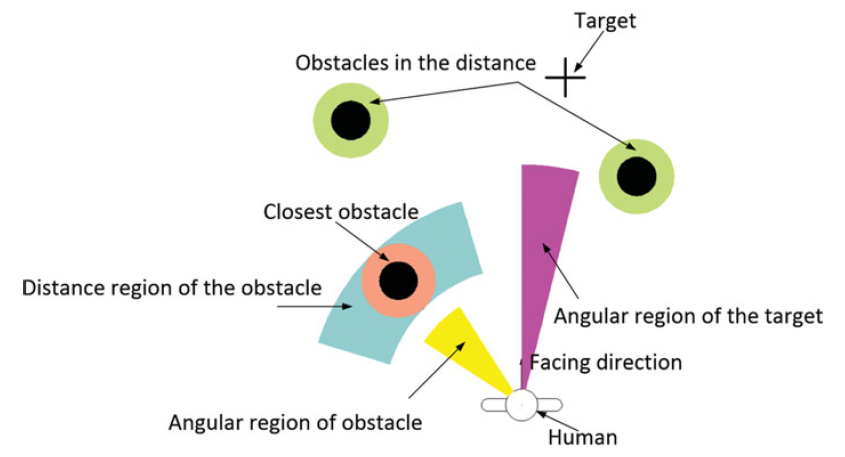
\includegraphics[width=0.3\textwidth]{hum.PNG}
	\caption{Human perception of the environment}
\end{figure}

According to the perception of ourself to find a target in unknown space, we want to use the position information of the target and the nearest obstacle to define our robot state.

First we define the heading direction of our robot, which is the moving direction when our robot goes forward. Then define the forward area of our robot. Setting the heading direction be y-axis positive direction and the robot center be origin, construct a planner coordinate system and let the right to be the positive direction of x-axis, the I and II quadrant is the forward area of our robot. This is because our camera can see such scope. Then, we divide the forward area to 10 parts on average. As the figure below, the state of the nearest obstacle angular position is A1 - A10.

Next we define the safe and unsafe area. As is shown in the figure below,there are three region in the forward area with radius R1-R3. When our robot find no obstacle inside R3, we say it is in safe region, otherwise it is in the unsafe region. The policies in the 2 region are different we will talk about it later. For unsafe region, we separate it into 3 region, whose radius are R1-R3. So there are 3 state for robot in unsafe region.
\begin{figure}[H]
	\centering
	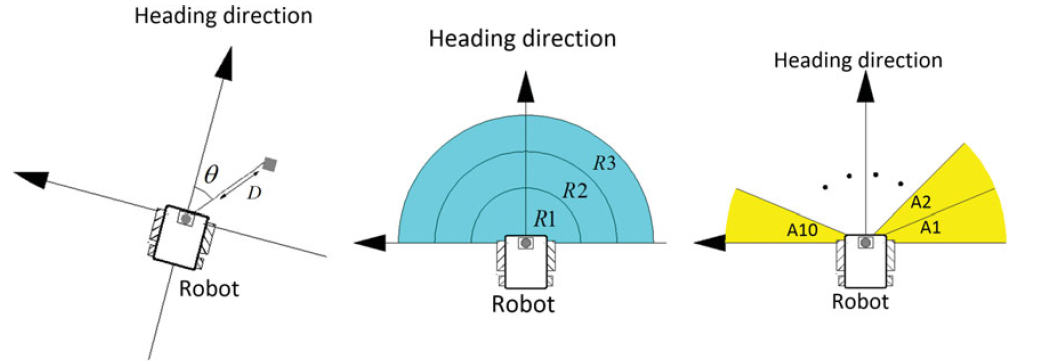
\includegraphics[width=0.4\textwidth]{ra.PNG}
	\caption{State definition for robot's nearest obstacle}
\end{figure}
Then, we define the target angular state of our robot. As in shown in the figure below, we divide the whole plan into 8 parts on average. So there will be 8 states in the target angular state.
\begin{figure}[H]
	\centering
	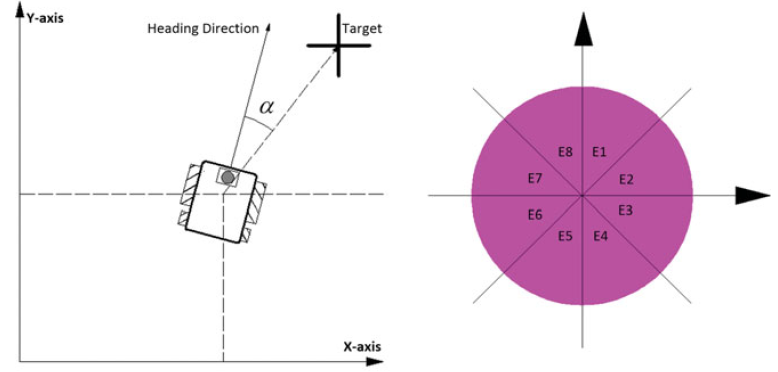
\includegraphics[width=0.4\textwidth]{re.PNG}
	\caption{State definition for robot's target}
\end{figure}
	We also consider the robot's current linear and angular velocity and add them into the state. We just divide the linear velocity(Vl) into 4 segments on average and the angular velocity(Va) into 10 segments on average, which can be represent by the following equations:
	\begin{equation}
	VL=\left\{
	\begin{array}{rcl}
	VL_1 & & {Vl \in [0,Vl_{max} / 4)}\\
	VL_2 & & {Vl \in [Vl_{max} / 4,2Vl_{max} / 4)}\\
	VL_3 & & {Vl \in [2Vl_{max} / 4,3Vl_{max} / 4)}\\
	VL_4 & & {Vl \in [3Vl_{max} / 4,Vl_{max}]}
	\end{array} \right.
	\end{equation}
	\begin{equation}
	VA=\left\{
	\begin{array}{rcl}
	VA_1 & & {Va \in [-Va_{max},-Va_{max}+Va_{max}/5)}\\
	VA_2 & & {Va \in [-Va_{max}+Va_{max}/5,-Va_{max}+2Va_{max}/5)}\\
	\vdots & & {\vdots}\\
	VA_{10} & & {Va \in [-Va_{max}+9Va_{max}/5,Va_{max}]}
	\end{array} \right.
	\end{equation}
	Using all the definitions above, the state at any time instant
	can be completely defined as a combination of the approximate regions of the closest obstacle ahead,
	the target and the linear and angular velocity: $$s_t = (R,A,E,VL,VA)$$ where $s_t$ is the state of robot at time instant t , R is the distance region of obstacle, A is the angular region of obstacle, E is the angular region of the goal andVL andVA are the velocity region of linear
	velocity and angular velocity, accordingly.
	
	\subsection{Definition of reward function}
	To define the reward function, two transient states and two terminal states
	should be introduced. All these states are defined as the transition state S.
	
	Two transient states are defined as:
	\begin{itemize}
		\item The safe states(SS) if the robot is in safe region.
		\item The non-safe states (NS) if the robot is in unsafe region.
	\end{itemize}

	Two terminal states are defined as:
	\begin{itemize}
		\item The win state (WS) if the robot reaches its goal.
		\item The fail state (FS) if the robot collided with the obstacle. 
	\end{itemize}

	In order to let the robot navigate safely as well as get its target, we define the reward function as follows:
	\begin{itemize}
		\item $R(s_t,a_t) = 1$ for moving from NS to SS.
		\item $R(s_t,a_t) = -1$ for moving from NS to FS.
		\item $R(s_t,a_t) = 2$ for moving from NS to WS.
		\item $R(s_t,a_t) = a*D_{obs} + b * \alpha_{tar} + c* v_t$ for moving from NS to NS.
	\end{itemize}
	For moving form NS to NS,$D_{obs}$ is the distance to the nearest obstacle , $\alpha_{tar}$ is the angle  between the heading direction and the target direction and $v_t$ is the current linear velocity.Since we want to use this function to decide whether the move is good or not.
	To summarize, the reward function can be rewritten as :
	\begin{equation}
	R(s_t,a_t)=\left\{
	\begin{array}{rcl}
	1 & & {NS \rightarrow SS}\\
	-1 & & {NS \rightarrow FS}\\
	2 & & {NS \rightarrow WS}\\
	a*D_{obs} + b * \alpha_{tar} + c* v_t & & {NS \rightarrow NS}
	\end{array} \right.
	\end{equation}
	
	\subsection{Value function}
	The value function of Q-learning algorithms is stored in a table. The rows of the table represent
	different states the robot passes through, and the columns are the actions performed by the robot. All
	the Q-values stored in the table are initially set to zero. During the training process, each entry in
	the table is filled by updating Q-values of state and action pairs. The update equation for Q-learning
	algorithm is as follows:$$Q(s_t,a_t) = Q(s_t,a_t) + \beta(R(s_t,a_t) + \gamma max_a Q(s_{t+1},a) - Q(s_t,a_t))$$
	where $s_t$ and $a_t$ are the state and action that robot takes at time $t$ . $\beta$ is the learning factor. $\gamma$ is the	discount factor. $max_a Q(s_{t+1},a)$ is the maximum Q-value calculated for taking all possible actions in
	the new state at time t + 1. By exposing the robot in different training scenarios, the Q-table of the
	robot is updated. After training the robot, it is able to navigate in a real environment using information
	stored in the table.
	
	\subsection{Defining actions by a dynamic window -- making the trajectory smooth}
	Since all states space have been defined completely, allowed actions for each state can be specified.
	Action is defined as the index from which the pair of linear and angular velocity can be calculated.
	At any time, velocities that a robot can reach are in a dynamic window, which restricts the
	admissible velocities to those that can be reached within a short time interval when the limited
	accelerations of the robot are given.
	\begin{figure}[H]
		\centering
		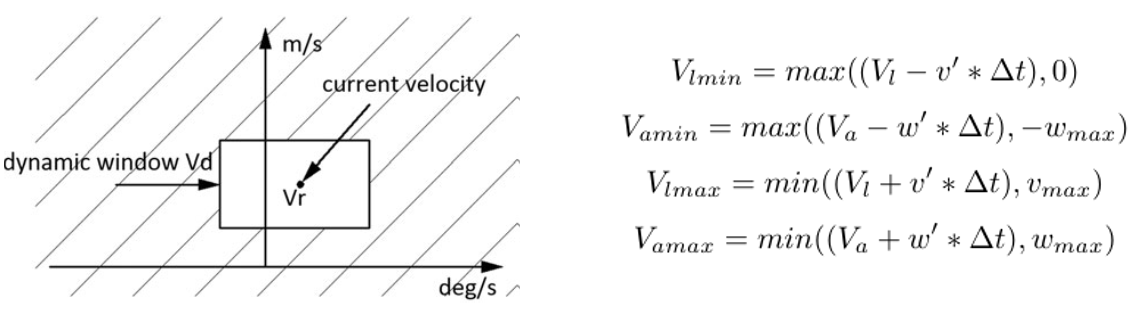
\includegraphics[width=0.4\textwidth]{dym.PNG}
		\caption{Dynamic window}
		\label{dym}
	\end{figure}
	As shown in \ref{dym}, the current velocity of the robot is $Vr = (Vl ,Va )$.Vl and Va are the linear and
	angular velocity, respectively. The dynamic window Vd for the current velocity can be described as
	follow: $$Vd = \{(v,w) | [Vl-v'*\Delta t, Vl+v'*\Delta t] \bigwedge [Va-w'*\Delta t, Va+w'*\Delta t],$$ $$ 0< v < v_{max},w<w_{max} \}$$
	In our design, each state has 40 actions to choose. In other words, the index has the range from
	1 to 40. As angular and linear velocities in Vd are continuous, the resolution of velocity should
	be introduced. Resolutions for linear and angular velocity are $res_l = (Vl_{max} - Vl_{min} )/4$ and $res_a =
	(Va_{max} - Va_{min} )/10$, respectively.
	
	The linear velocity $Vnl$ and angular velocity Vna calculated from the action taken, i.e. index n, $n \in
	[1, 40]$ are defined as follow:
	\begin{equation}
	\label{act}
	\left\{
	\begin{array}{rcl}
	Vnl = Vl_{min} + floor((n-1)/4)*res_l & & {}\\
	Vna = Va_{min} + ((n-1)mod10)*res_a & & {}
	\end{array} \right.
	\end{equation}
	
	\subsection{The calculation of robot movement and the introduction of virtual trajectory}
	Let $[P_{xt},P_{yt},\theta_{Rt}]^T$ denotes the position and heading direction of robot at time t in a global coordinate
	system. Let $[v_t,w_t]^T$ denote the pair of linear and angular velocity calculated from the action taken
	at time t . The position and heading direction of robot  $[P_{x(t+1)},P_{y(t+1)},\theta_{R(t+1)}]^T$ at time t + 1 can be
	calculated as follow:
	\begin{figure}[H]
		\centering
		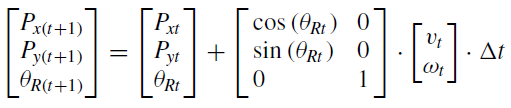
\includegraphics[width=0.3\textwidth]{vt.PNG}
	\end{figure}
	$\Delta t$ is the time interval between t + 1 and t . As the time interval is quite short, the
	movement of robot is not quite noticeable for evaluation. In order to properly define a reward function,
	the result of a taken action should be ‘magnified’. Therefore, a virtual trajectory should be introduced
	using simulation time $t_s$. The virtual trajectory is defined as a hypothetical route which the robot
	generates in simulation time $t_s$ by the pair of linear and angular velocity $[v_t,w_t]^T$.The position and
	heading direction of robot $[P_{xv},P_{yv},\theta_{Rv}]^T$ at the end of virtual trajectory can be achieved by iterating the above equation. 
	The pseudo code that illustrates the iterative process is as follows.
	\begin{algorithm}
		\caption{Virtual trajectory iteration}
		function Iterative-trajectory($P_{xt},P_{yt},\theta_{Rt},v_t,w_t$)
		
		persistent: $\Delta t$ the time interval between time t and t+1, $t_s$ the simulation time to generate a virtual trajectory.
		
		\For{counter=1 to $t_s / \Delta t$}{
			$P_{xt} = P_{xt} + v_t * cos(\theta_{Rt}*\Delta t)$
			
			$P_{yt} = P_{yt} + v_t * sin(\theta_{Rt}*\Delta t)$
			
			$\theta_{Rt} = \theta_{Rt} + w_t * \Delta t$
		} 
		$P_{xv} = P_{xt}$
		
		$P_{yv} = P_{yt}$
		
		$\theta_{Rv} = \theta_{Rt}$
		
		return $P_{xv},P_{yv},\theta_{Rv}$
	\end{algorithm}
	
	\subsection{The policy}
	The policy for navigation in real world can be achieved by training the robot in different testing
	environments. In safe region, the robot simply turns to the target and moves closer. In non-safe region, however, the
	robot has to follow the policy when navigating. In this case, the robot takes the action with the highest
	Q-value from the Q-table for the current state, and moves forward with the pair of linear and angular
	velocity calculated from the action taken.
	
	\subsection{Training procedure for the Qlearning algorithm}
	Training the robot in different environments
	can update the Q-value stored in the Q-table. Every one of the training environments is called a
	scenario. Since the location of the closest obstacle is not given in advance, the robot is obliged to
	perceive and choose the closest obstacle ahead of it through sensors.
	\begin{figure}[H]
		\centering
		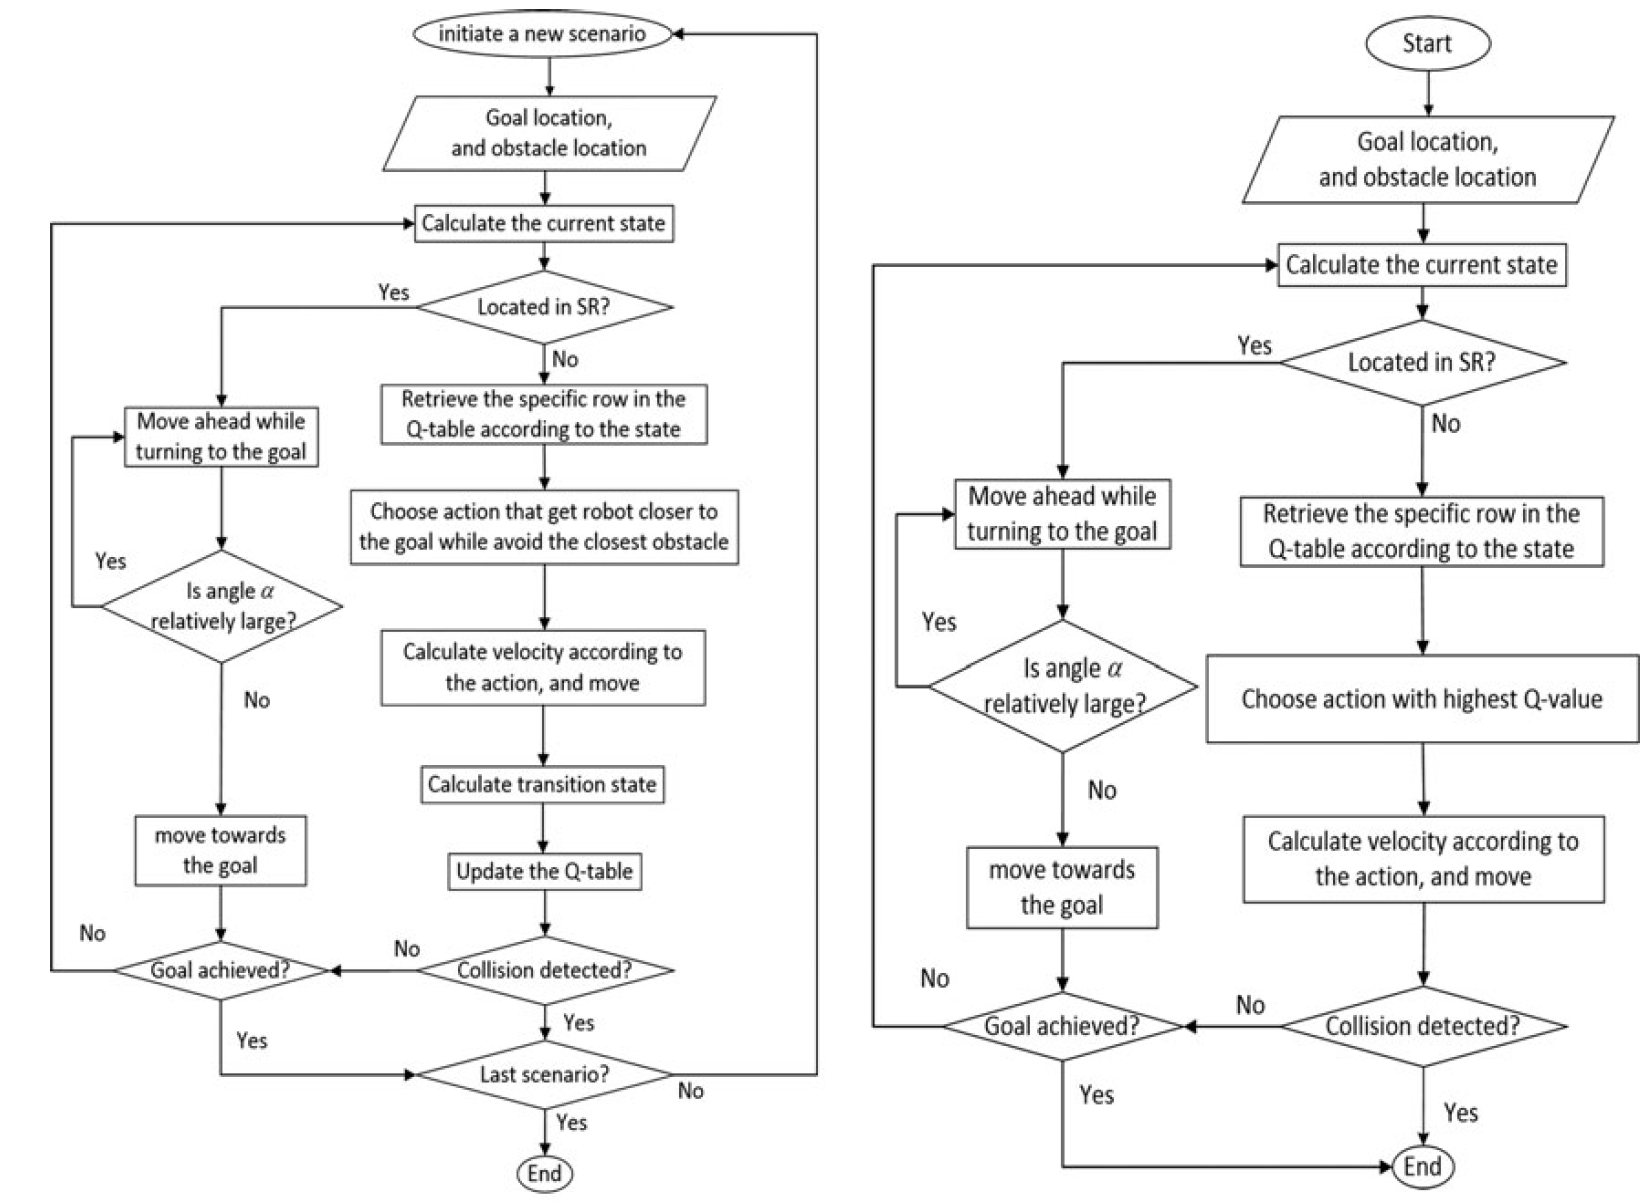
\includegraphics[width=0.5\textwidth]{tat.PNG}
		\caption{Training and testing flow chart}
		\label{flowchart}
	\end{figure}
	The flowchart of training procedure for the Q-learning algorithm is shown in the figure above.The training
	procedure contains different scenarios. Each scenario begins with calculating the robot current state.
	The location of the goal is defined in the global coordinate system and set to the robot. The location
	of obstacles and velocity of robot are achieved through the sensors equipped on the robot. Therefore,
	the state at time t, the current state of the robot can be calculated at this stage.
	
	Now that the state has been determined, it is easy to find out whether the robot is located in safe region by
	determining the approximate region where the closest obstacle in FA is located. If the robot is located
	in SR and if the angle between the heading direction and the target direction is relatively large, it will move closer to the target by a pair of linear and angular velocity $[v_f,w_f]^T$ or $[v_f,-w_f]^T$ depending on which pair of velocity
	can turn the robot to the target faster, and if the angle is relatively small, then the robot will move
	closer to the target by a pair of linear and angular velocity $[v_f,0]^T$. $v_f,w_f$ are the fixed linear
	and angular velocity. If the robot reaches the goal, then current training scenario will finish and a new
	scenario will initiate. Otherwise, the robot calculates the state at time t + 1 and repeats the process. 
	
	If the robot is located in non-safe region, it has to retrieve the specific row in the Q-table according to the
	state calculated, and choose the action that will make it move closer to the goal while avoiding the
	closest obstacle. As mentioned before, the action chosen is actually an index. The robot can calculate
	the pair of linear and angular velocity according to the index using Eq. \ref{act}. After moving towards
	the goal with the calculated velocity pair, the robot calculates the reward for the current transition
	state and updates the Q-table using the reward function and value iteration function.Then the robot will check if it has
	collided with the obstacle. If the collision happens, then robot will initiate a new scenario. Otherwise,
	the robot will check if it has reached the goal. If it has reached its goal, a new scenario will initiate, or
	the robot will repeat the current training process by calculating the state in a new time instant t + 1.
	\begin{figure}[H]
		\centering
		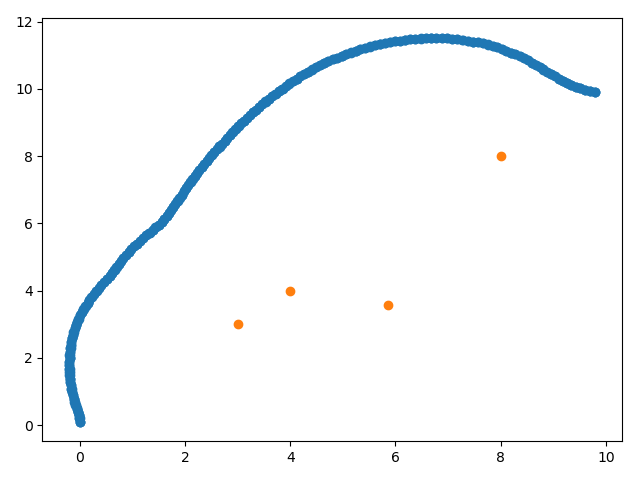
\includegraphics[width=0.3\textwidth]{train.PNG}
		\caption{One scenario of training,start from (0,0) and target is (10,10), the red dots are dynamic obstacles}
	\end{figure}
	\subsection{Navigation with the learned policy}
	After finishing the training process of our Qlearning algorithm, we use the trained Q-table to test our algorithm. The process is shown in Fig. \ref{flowchart}.Once the robot has determined its current state, it is
	able to find out whether it is located in safe region or not. If the robot is located in safe region, it will move closer
	to the goal through a strategy described above. If the robot is located in non-safe region, it will retrieve the row
	in the Q-table according to its state and choose the action with the highest Q-value. After the pair of
	linear and angular velocity is calculated according to the chosen action, the robot moves forward with that velocity pair. The robot will recalculate its current state and repeat the process until it reaches its goal or collides with an obstacle.
\section{Experiments}
\subsection{Dynamic Obstacles}
To get sufficient training, we also add dynamic obstacles to the environment. Each dynamic obstacle has its boundary of movement in the shape of a circle, determined by the location of circle center and the length of circle radius. All circle centers are located in a certain boundary regarding the initial position of car and target.

Each time each dynamic obstacle will take random linear velocity and angular velocity to move around. When a dynamic obstacle reaches its boundary, it will go directly back to its circle center to avoid getting out of its boundary, and once it reaches its circle center, it will start to take random actions again.
	\begin{figure}[H]
	\centering
	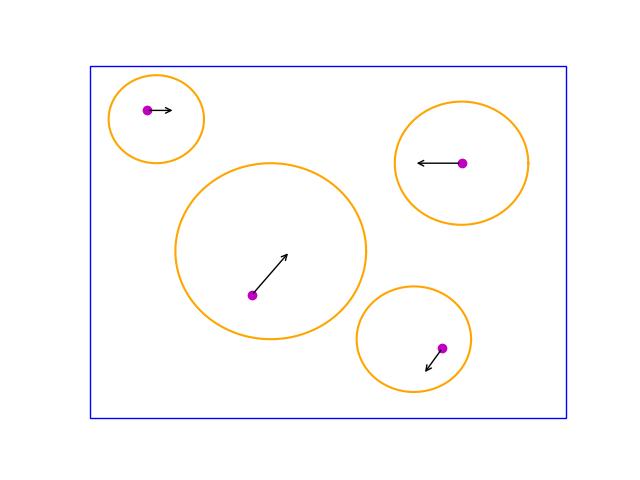
\includegraphics[width=0.3\textwidth]{fig1.PNG}
	\caption{Dynamic obstacles}
\end{figure}

\subsection{Simulation and Visualization}
For simulation, we just set a fixed time interval for the car and dynamic obstacles to update their position (static obstacles and target just stay still). Each time, dynamic obstacles take random actions at first, then the car will choose appropriate linear velocity and angular velocity to do updating based on its current observation in the environment and the policy learned during training. Making dynamic obstacles and the car moving simultaneously will bring more challenges, since it’s quite important to set a good observation rate for the car to know about the changing environment, which may be found by experiment, and this will be put into future work.

For visualization, we choose to use FuncAnimation in matplotlib. We maintain a graph containing the car, obstacles (both static and dynamic) and the target, and update the positions of dynamic obstacles and the car in graph every 0.05s (the trajectory of the car will also be recorded and shown). The animation stops when the car reaches the target.

\begin{figure}[H]
	\centering
	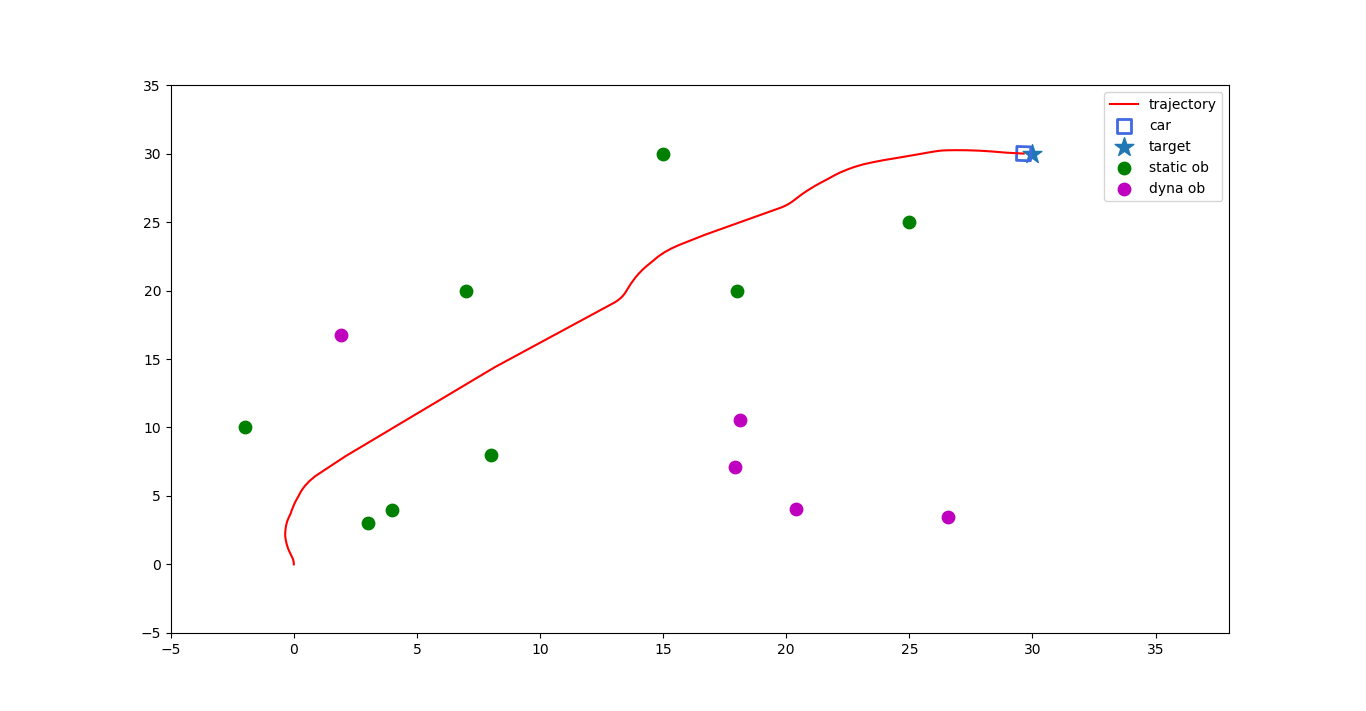
\includegraphics[width=0.3\textwidth]{fig2.PNG}
	\caption{Simulation and Visualization}
\end{figure}

\section{Conclusion}
In this course project, we designed a robot path planning method using Qlearning algorithm. We used human like perception to define the state of the robot. So the state are localized and not too complex, which is suitable for navigation in a dynamic environment. Then, we used a dynamic window to generate the actual linear velocity and angular velocity of the robot which will make the robot's trajectory more smooth. In the training process, we seperate the safe and non-safe region and applied different strategies in that two region. We only use Qlearning in non-safe region, which makes it more easy to train and closer to real world situations.

In addition, we create vitual dynamic environment to train and test our Qlearning training result. And the results shows that in an environment with static and dynamic obstacles, the robot can navigate well and its trajectory is smooth. So we think we did well in the course project.

For our future work, we want to use our method in the real world robot. And also improve our algorithm for real robot.
\appendix
% Bibliography
\bibliographystyle{plain}
\bibliography{tex}

\end{document}
% End of v2-acmtog-sample.tex (March 2012) - Gerry Murray, ACM
